\documentclass[reqno,a4paper,12pt]{amsart}

\usepackage{amsmath,amssymb,amsthm,geometry,xcolor,soul,graphicx}
%\usepackage{array}
\usepackage{float} % 在tcolorbox中添加table (由于tcolorbox已经是一个box,因此不能直接加table)
\usepackage{subfig} % 多张图放一起
\usepackage{titlesec}
%\usepackage{enumitem}
\usepackage{enumerate}
\usepackage{lipsum}
\usepackage{listings}
\allowdisplaybreaks[4] %align公式跨页
\RequirePackage[most]{tcolorbox}
\usepackage{braket}
%\usepackage{esint} %$\varoiint$ (带圈的二重积分)
%\usepackage[colorlinks,linkcolor=red]{hyperref} %\url{}超链接
\usepackage[scheme=plain,linespread=1,punct=CCT]{ctex}% Chinese support, single line space, narrow-version SBC case punctuations
\setCJKfamilyfont{zhsong}[AutoFakeBold={2.17}]{SimSong-Regular}
\renewcommand{\songti}{\CJKfamily{zhsong}}
%\usepackage{xeCJK}
%\setCJKmainfont{Kai}
\geometry{left=0.7in, right=0.7in, top=1in, bottom=1in}

\renewcommand{\baselinestretch}{1.3}

\title{固体物理第十一次作业}
\author{董建宇 ~~ 2019511017}

\begin{document}

\maketitle

\begin{enumerate}[1.]

\item \textbf{(16.1) Metals and Insulators} \\
Explain the following: \\
(a) sodium, which has two atoms in a bcc (conventional cubic) unit cell, is a metal; \\
(b) calcium, which has four atoms in a fcc (conventional cubic) unit cell. is a metal; \\
(c) diamond, which has eight atoms in a fcc (conventional cubic) unit cell with a basis, is an electrical insulator, whereas silicon and germanium, which have similar structures, are semiconductors. (Try to think up several possible reasons!) \\
$\triangleright$ Why is diamond transparent? 
\begin{tcolorbox}[breakable, colback = black!5!white, colframe = black]
\begin{enumerate}[(a)]
\item 对于传统晶包为体心立方的钠而言,原初晶包中只含有1个钠原子,每个钠原子提供一个价电子,因此第一布里渊区只填充了一半的电子,因此钠是金属。

\item 对于传统晶包为面心立方的钙而言,原初晶包中只含有1个钙原子,但每个钙原子可以提供2个价电子,但是钙的能带结构表明:价带与导带出现交叠,也就意味着所有的电子部分填充在价带,部分填充在导带,因此价带和导带均为部分填充,所以钙是金属。 
\begin{figure}[H]
	\centering
	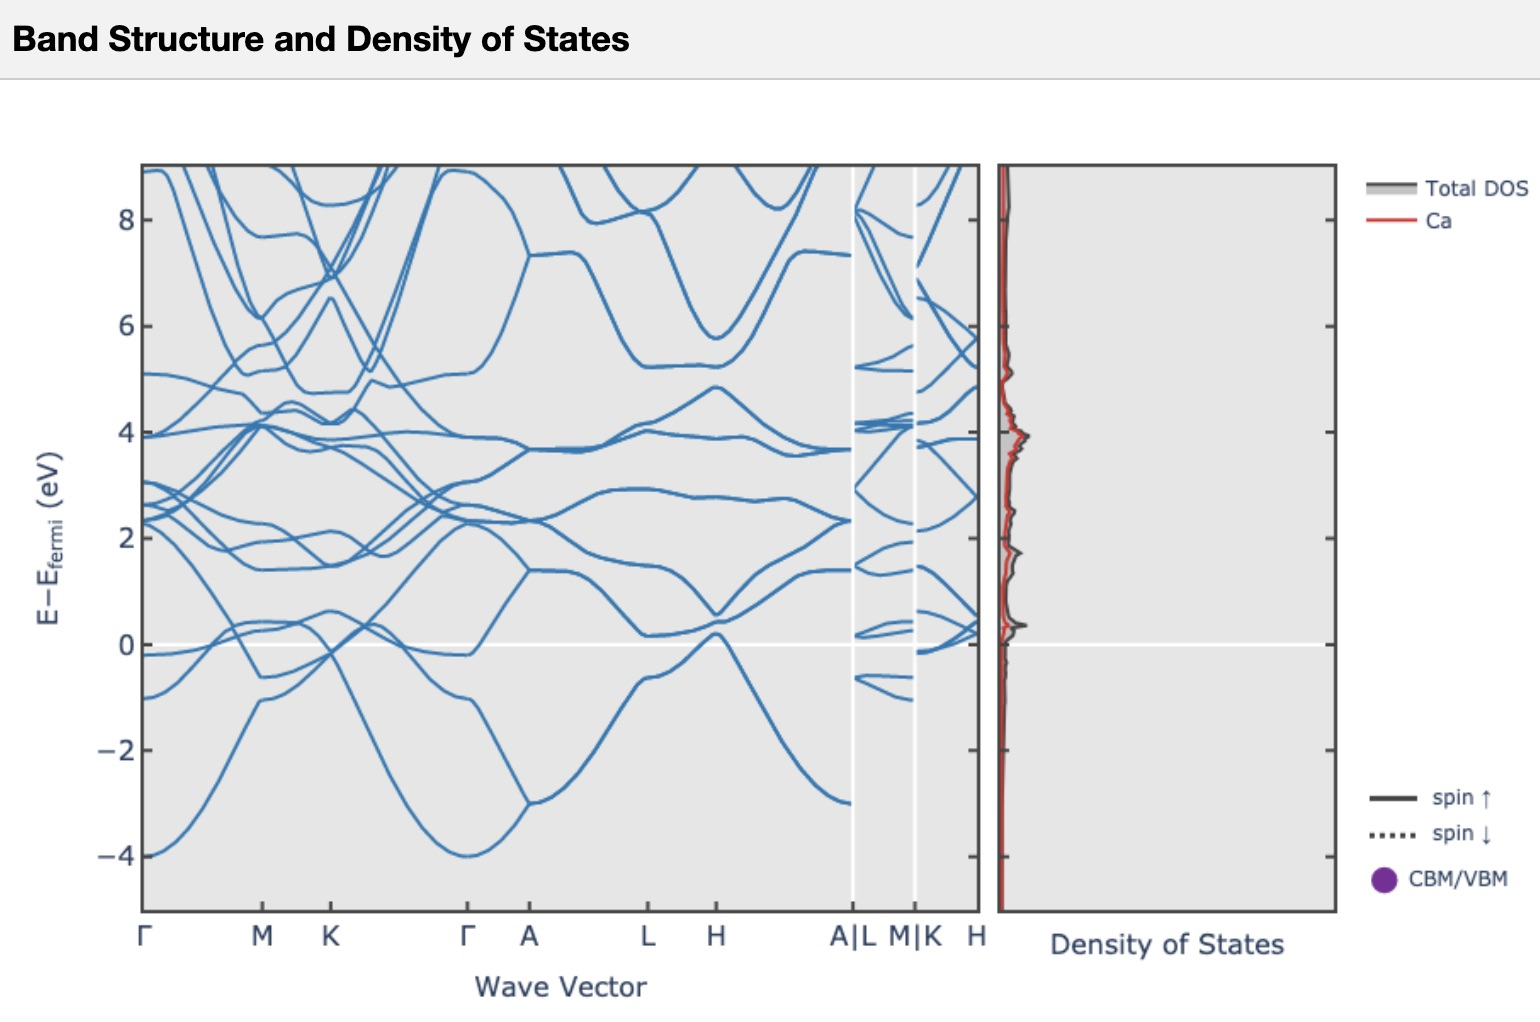
\includegraphics[width = 120mm]{Ca-band-structure.jpeg}
	\caption{Ca的能带结构与态密度}
\end{figure}

\item 对于金刚石,每个原初晶包中包含2个碳原子,每个碳原子可以提供四个电子,因此可以完全填充满4个能带,同时,由于其带隙较大,所以是绝缘体。而对于硅和锗,由于其带隙较小(小于4eV),所以是半导体。
\begin{figure}[H]
	\centering
	\subfloat[C]{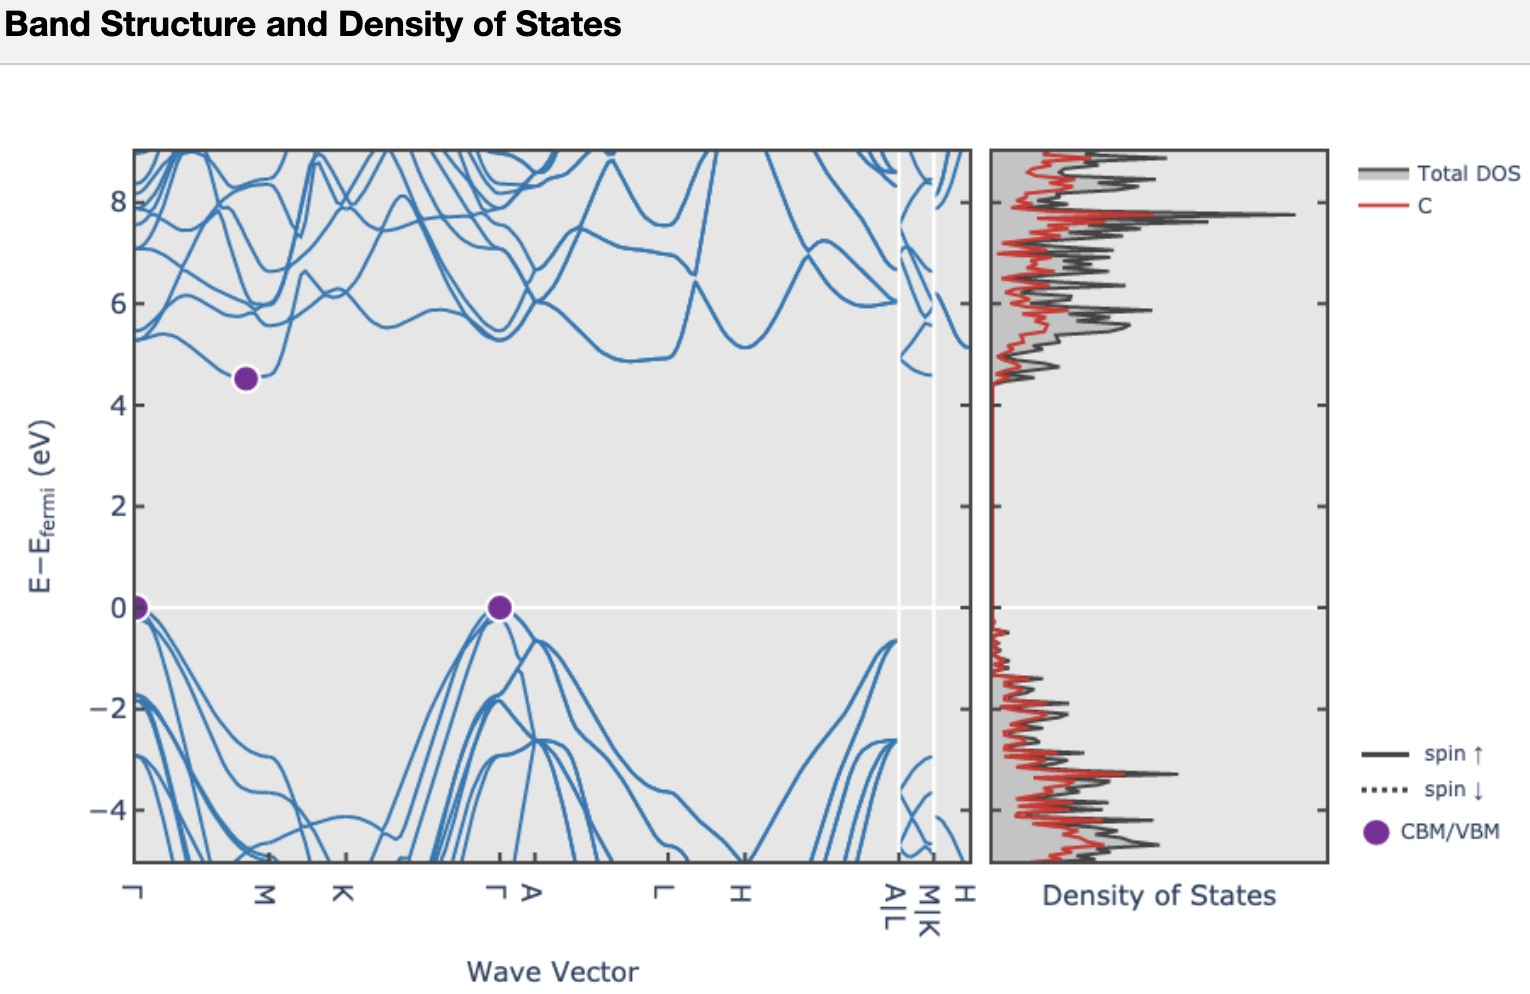
\includegraphics[width  = 47mm]{C-band-structure.jpeg}} \hspace{2pt}
	%\caption{C的能带结构与态密度}
	\subfloat[Si]{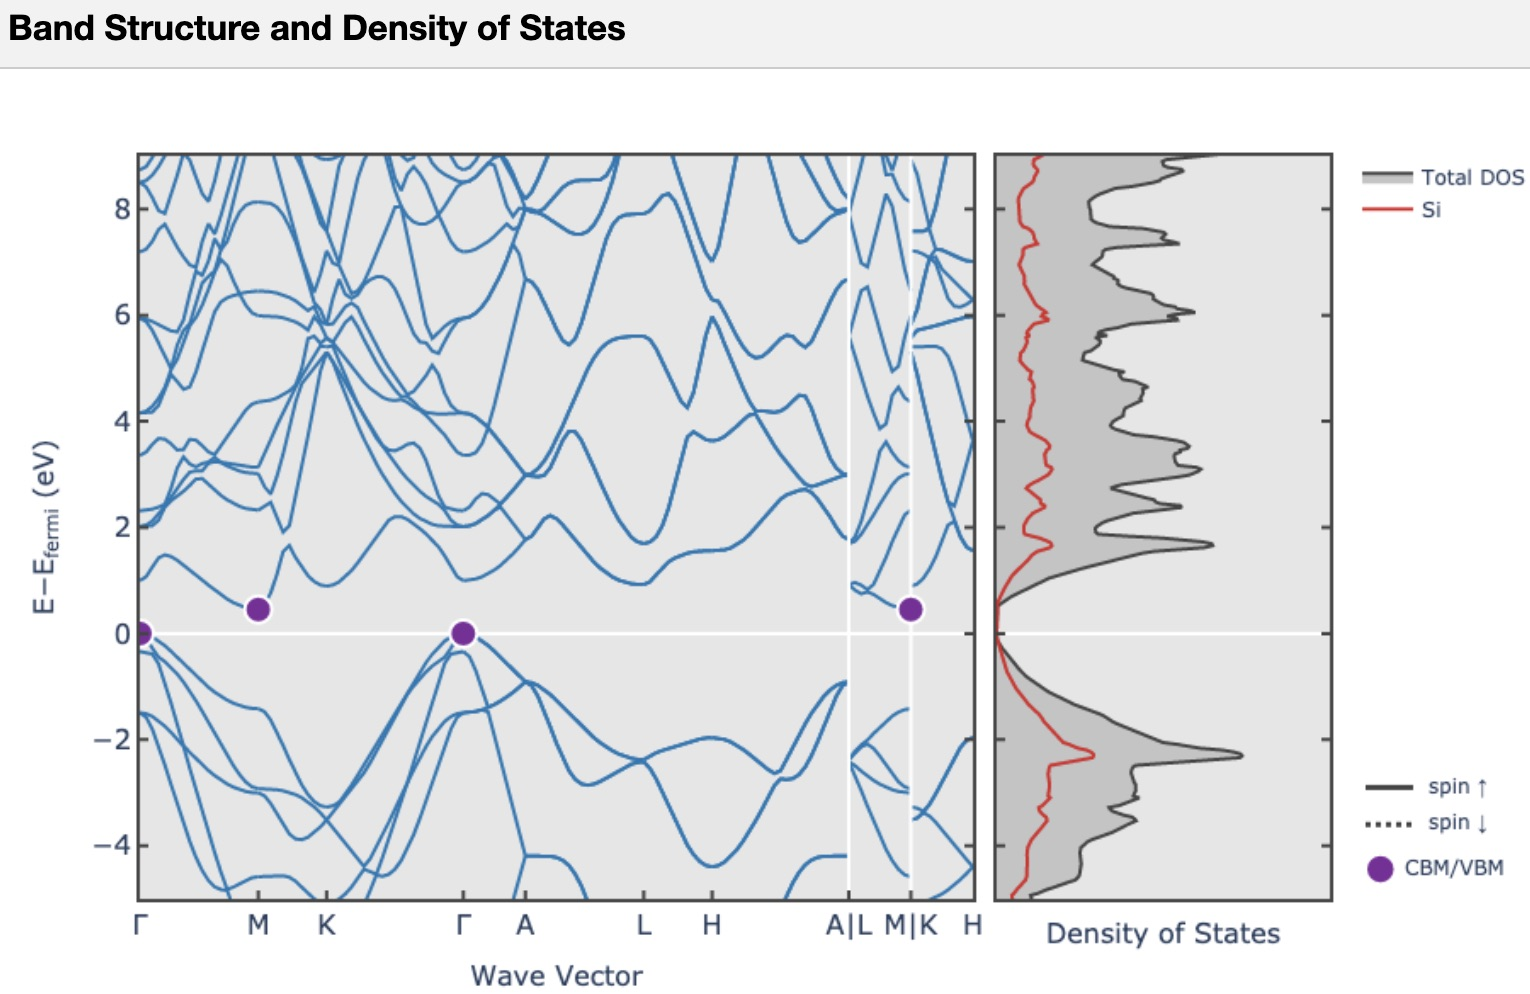
\includegraphics[width  = 47mm]{Si-band-structure.jpeg}} \hspace{2pt}
	\subfloat[Ge]{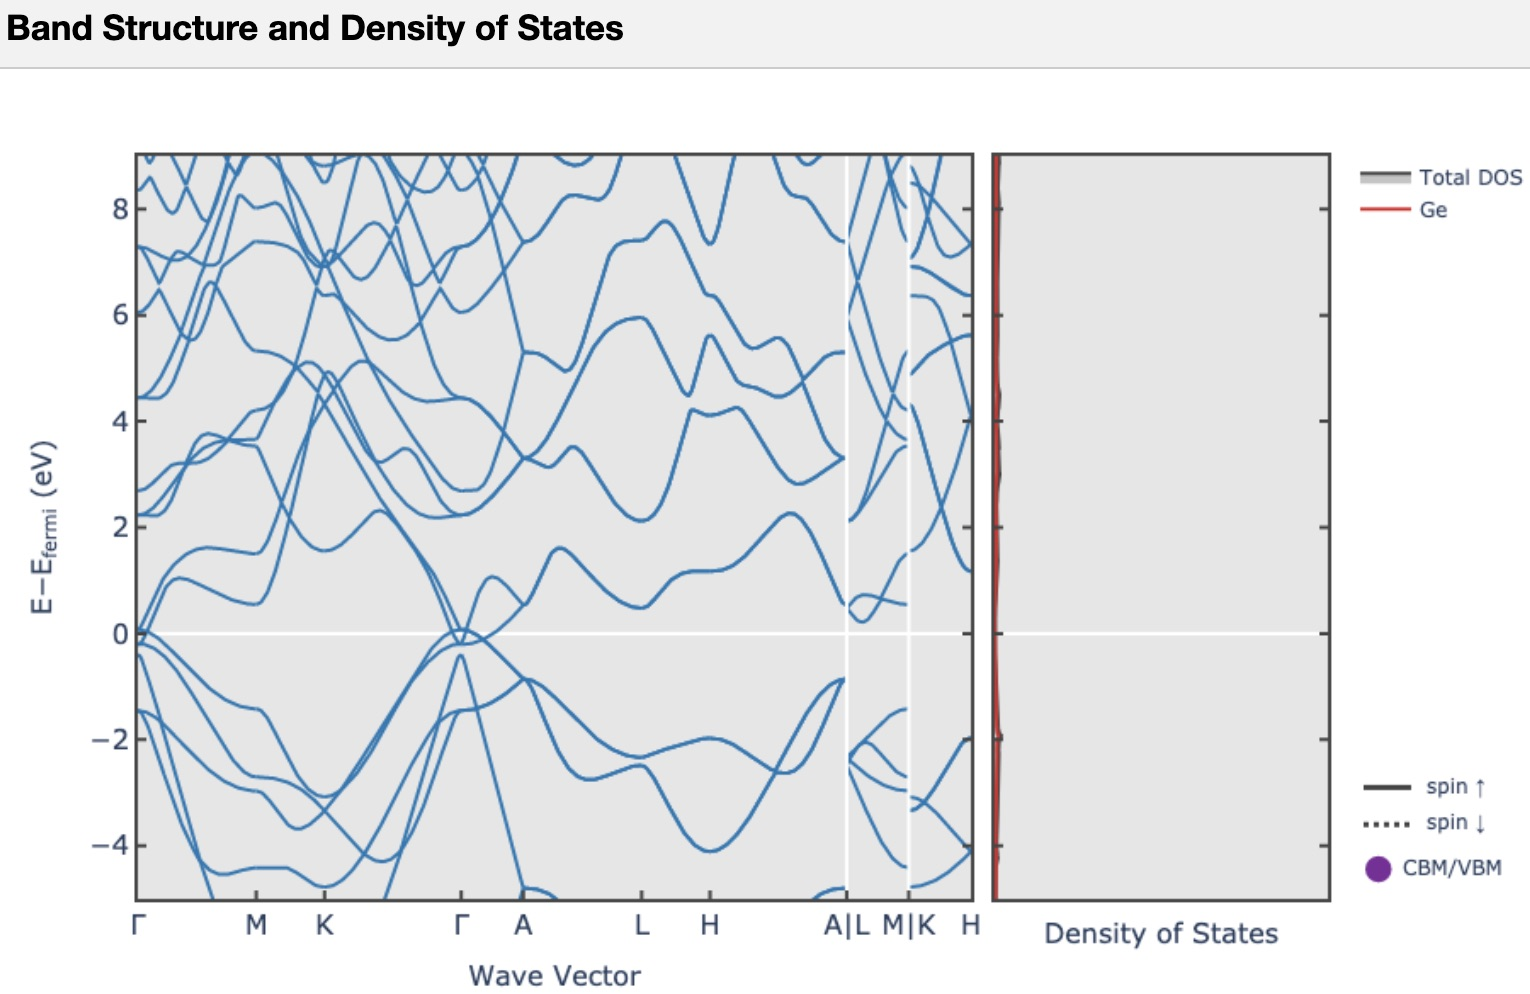
\includegraphics[width  = 47mm]{Ge-band-structure.jpeg}}
	\caption{不同物质的能带结构与态密度}
\end{figure}
Materials Project数据库中查到三种物质带隙分别为:
\begin{table}[H]
\centering
\begin{tabular}{|l|l|l|l|}
\hline
物质 & C & Si & Ge \\ \hline
带隙(eV) & 4.525 & 0.514 & 0.086 \\ \hline
\end{tabular}
\end{table}
原因可能为: \\
$\bullet$ 原子序数较小的原子核对核外电子束缚较紧,从而使得核外电子受激发跃迁至导带从而实现导电。因此碳的带隙大于硅的带隙大于锗的带隙。 \\
$\bullet$ 在紧束缚近似下,考虑单原子模型,能级越高的两相邻能级的能量差减小,因此随着核外电子层数(主量子数)的增加,带隙减小。因此碳的带隙大于硅的带隙大于锗的带隙。 \\
$\triangleright$ 金刚石透明是因为其带隙高于可见光能量(1.5eV~3eV),因此使用可见光照射金刚石并不会产生激发,即不会有可见光被吸收,也就意味着金刚石是透明的。
\end{enumerate}
\end{tcolorbox}

\item \textbf{(16.2) Fermi Surface Shapes} \\
(a) Consider a tight binding model of atoms on a (two-dimensional) square lattice where each atom has a signle atomic orbital. If these atoms are monovalent, describe the shape of the Fermi surface. \\
(b) Now suppose the lattice is not square, but is rectangular instead with primitive lattice vectors of length $a_x$ and $a_y$ in the $x$ and $y$ directions respectively, where $a_x>a_y$. In this case, imagine that the hoppings have a value $-t_x$ in the $x$-direction and a value $-t_y$ in the $y$-direction, with $t_y>t_x$. (Why does this inequality match $a_x>a_y$?) \\
$\triangleright$ Write an expression for the dispersion of the electronic states $\epsilon(\mathbf{k})$. \\
$\triangleright$ Suppose again that the atoms are monovalent, what is the shape of the Fermi surface now?
\begin{tcolorbox}[breakable, colback = black!5!white, colframe = black]
\begin{enumerate}[(a)]
\item 对于紧束缚近似下的二维晶格,Hamiltonian可以写为:
\[
	\hat{H} = \frac{\hat{p}^2}{2m} + \hat{V}_{mn} + \sum_{i\neq m, j\neq n} \hat{V}_{ij}.
\]
则在紧束缚近似下可以假设
\[
	\bra{m',n'} \sum_{i\neq m, j\neq n}\hat{V}_{ij} \ket{m,n} = \left\{ \begin{array}{ll}
		V_0, & m' = m,~n'=n; \\
		-t, & \vert m'-m \vert + \vert n'-n \vert = 1; \\
		0, & otherwise.
	\end{array} \right.
\]
假设任意一个态可以写为:
\[
	\ket{\psi} = \sum_m\sum_n \phi_{mn}\ket{m,n}.
\]
则可以计算Sch{\"o}rdinger方程为:
\[
	-t\phi_{m-1,n} - t\phi_{m,n-1} + (\epsilon_0+V_0) \phi_{m,n} - t\phi_{m+1,n} - t\phi_{m,n+1} = E\phi_{m,n}.
\]
则可以假设
\[
	\phi_{m,n} = e^{-i(mak_x+nak_y)}.
\]
其中$a$为正方形晶格的晶格常数。代入上式可得:
\[
	E = (\epsilon_0+V_0) - 2t(\cos(ak_x) + \cos(ak_y)).
\]
\begin{figure}[H]
	\centering
	\subfloat{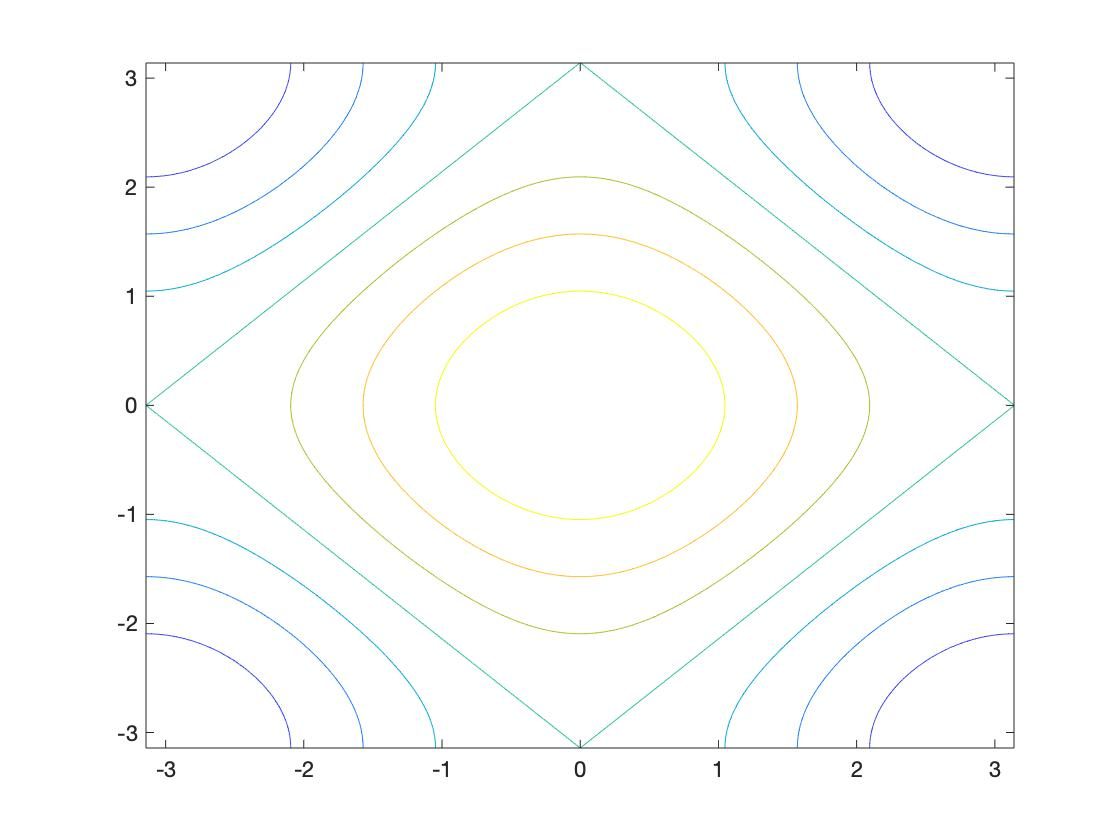
\includegraphics[width = 60mm]{16.2a.jpg}} \hspace{2em}
	\subfloat{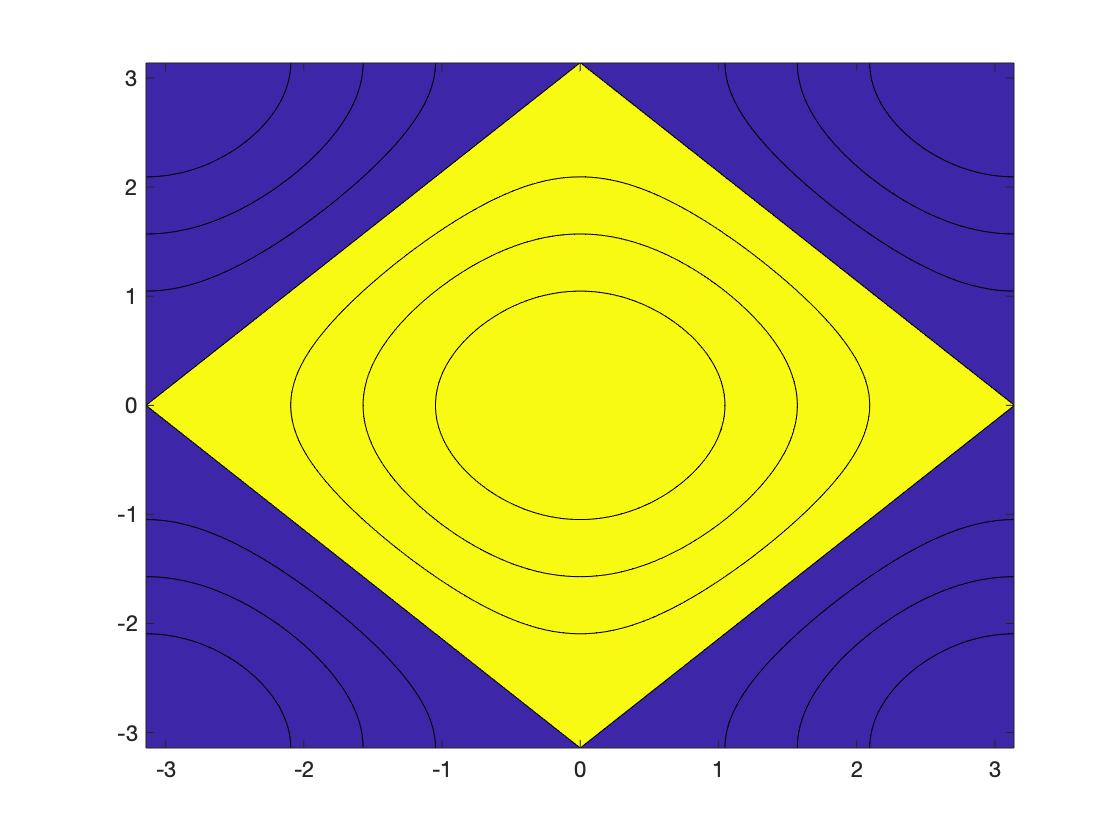
\includegraphics[width = 60mm]{16.2a2.jpg}}
	\caption{\text{色散关系与费米面}}
\end{figure}
\textcolor{blue}{右图中黄色区域内为一个元胞中的费米面。}

\item 对于长方形晶格,晶格常数大的方向原子间距较大,也就意味着相邻两个态之间的交叠较小,则当$a_x>a_y$时,沿$x$方向的原子间距大,则有$-t_x>-t_y$,即$t_y>t_x$。 \\
$\triangleright$ 对于长方形晶格,需要对紧束缚近似下非对角元修改如下:
\[
	\bra{m',n'} \sum_{i\neq m, j\neq n}\hat{V}_{ij} \ket{m,n} = \left\{ \begin{array}{ll}
		V_0, & m' = m,~n'=n; \\
		-t_x, & m' = m\pm 1, ~ n' = n; \\
		-t_y, & m' = m, ~ n' = n \pm 1; \\
		0, & otherwise.
	\end{array} \right.
\]
则Sch\"ordinger方程可化为:
\[
	-t_x\phi_{m-1,n} - t_y\phi_{m,n-1} + (\epsilon_0+V_0)\phi_{m,n} - t_x\phi_{m+1,n} - t_y\phi_{m,n+1} = E\phi_{m,n}.
\]
则可以假设:
\[
	\phi_{m,n} = e^{-i(ma_xk_x + na_yk_y)}.
\]
可得色散关系为:
\[
	E = \epsilon_0+V_0 - 2t_x\cos(a_xk_x) - 2t_y\cos(a_yk_y).
\]
$\triangleright$ 取$t_y = 2t_x = 2$, $a_x/2 = a_y = 1$,绘图如下:
\begin{figure}[H]
	\centering
	\subfloat{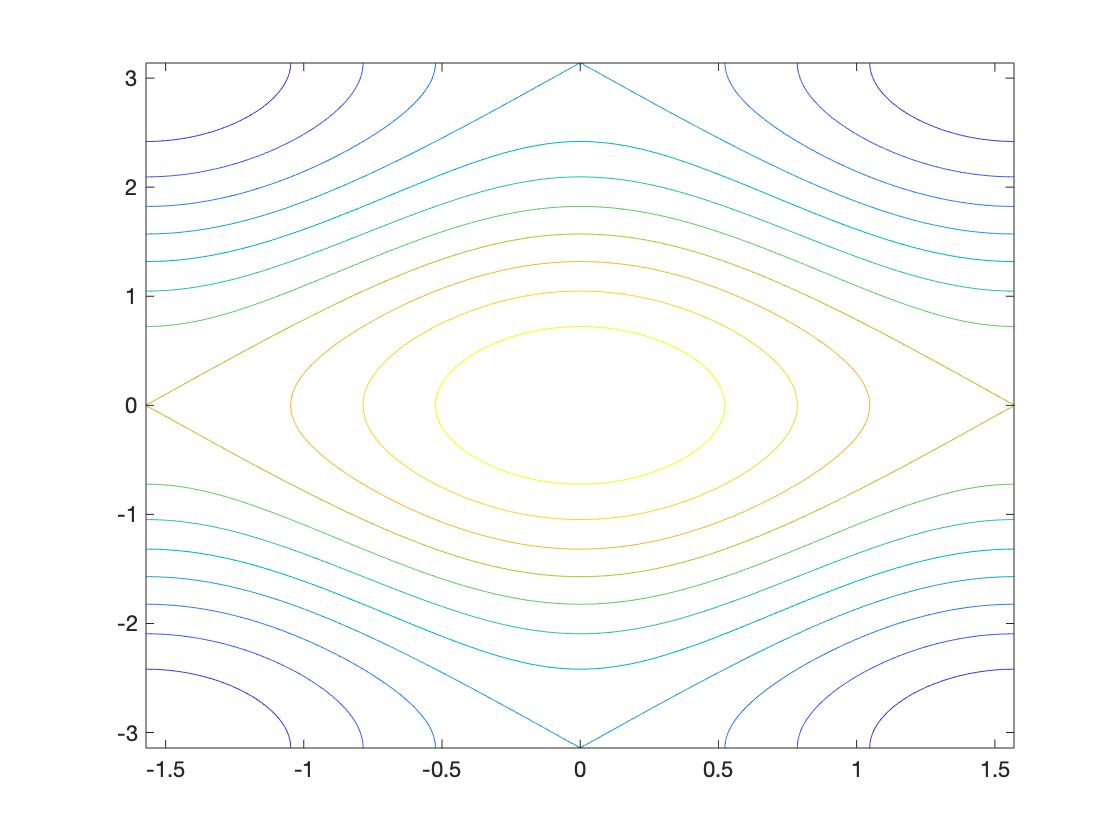
\includegraphics[width = 60mm]{16.2b.jpg}} \hspace{2em} 
	\subfloat{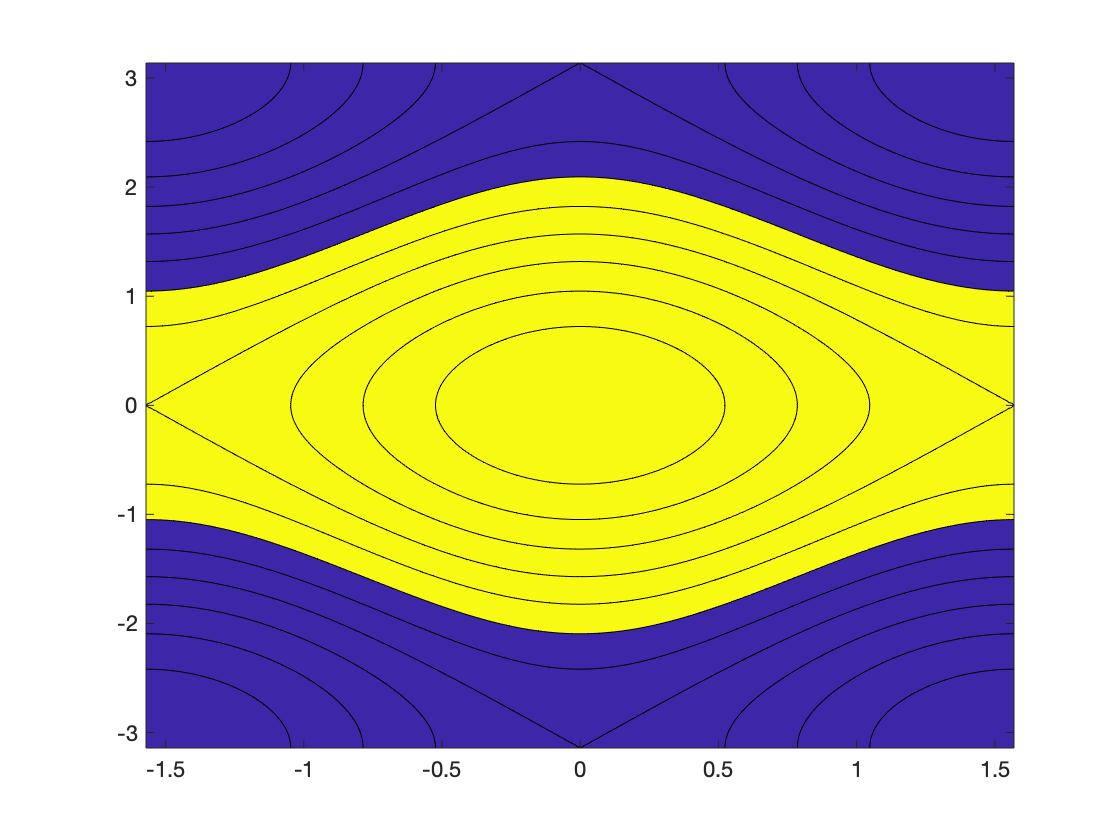
\includegraphics[width = 60mm]{16.2b2.jpg}}
	\caption{\text{色散关系与费米面}}
\end{figure}
\textcolor{blue}{右图中黄色区域内为一个元胞中的费米面。}

\end{enumerate}
\end{tcolorbox}

\item \textbf{(17.1) Holes} \\
(a) In semiconductor physics, what is meant by a hole and why is it useful? \\
(b) An electron near the top of the valence band in a semiconductor has energy 
\[
	E = -10^{-37}\vert \vec{k} \vert^2
\]
where $E$ is in Joules and $k$ is in $m^{-1}$. An electron is removed from a state $\mathbf{k} = 2\times 10^8 m^{-1}\hat{x}$, where $\hat{x}$ isn the unit vector in the $x$-direction. For a hole, calculate (and give the sign of!) \\
(i) the effective mass (ii) the energy (iii)the momentum (iv) the velocity. \\
$\triangleright$ If there is a density $p = 10^5m^{-3}$ of such holes all having almost exactly this same momentum, calculate the current density and its sign.
\begin{tcolorbox}[breakable, colback = black!5!white, colframe = black]
\begin{enumerate}[(a)]
\item 空穴是价带中缺失的电子。描述少量的空穴的动力学过程可以等价地描述大量的电子的动力学过程,因此空穴是非常有用的。

\item 
\begin{enumerate}[(i)]
\item 有效质量为:	
\[
	m^* = -\frac{\hbar^2}{\nabla_{\vec{k}}^2 E} = 0.061m_e.
\]
有效质量为正值。
\item 能量为:
\[
	E_h = -E(\mathbf{k}) = 4\times 10^{-21}J \approx 0.025eV.
\]
能量为正值。
\item 动量为:
\[
	\vec{p}_h = -\hbar \vec{k} = -1.33\times 10^{-25}\hat{x} ~ kg\cdot m /s
\]
动量为负值,即空穴沿x轴负方向运动。
\item 速度为:
\[
	\vec{v}_h = \frac{\nabla_{\vec{k}}E}{\hbar} = -3.793 \times 10^{5}\hat{x} m/s.
\]
速度为负值,即速度方向沿x轴负方向。 
\end{enumerate}

$\triangleright$ 电流密度为:
\[
	\vec{J} = pe\vec{v} = 6.07 \times 10^{-9} \hat{x} A/m^2.
\]
即电流密度沿x轴负方向,大小为$6.07 \times 10^{-9} A/m^2$.
\end{enumerate}
\end{tcolorbox}

\item \textbf{(17.6) More Semiconductors} \\
Outline the absorption properties of a semiconductor and how these are related to the band gap. Explain the significance of the distinction between a direct and an indirect semiconductor. What region of the optical spectrum would be interesting to study for a typical semiconducting crystal?
\begin{tcolorbox}[breakable, colback = black!5!white, colframe = black]
半导体的光吸收是指吸收一个光子然后将能量转化为电子的能量从而将价带电子激发到导带。在这个过程中需要满足能量、动量守恒。因此需要光子能量大于带隙,才可以将价带电子激发到导带上并且满足能量守恒。针对动量守恒的条件,将带隙分为了直接带隙和间接带隙。其中直接带隙在电子受激发从价带跃迁至导带前后动量不变,因此很容易被激发(只需要光子能量大于带隙就可以);而对于间接带隙,由于光子波长相对于晶格常数很大,因此光子动量很小,则电子激发需要伴随声子的吸收或发射从而满足动量守恒条件。\\
对于不纯或者存在缺陷的半导体,在其原本的带隙中可能存在其他的态,因此可以在其带隙能量以下发生少量吸收;同时在非常弱的非线性过程中可以允许多个光子被吸收而只激发单个电子。 \\
半导体带隙一般在可见光至红外波段;只有较少数的半导体带隙达到蓝光甚至紫外波段。因为传统认为带隙小于$4eV$才为半导体,可见光范围约是$1.5eV\thicksim 3eV$。
\end{tcolorbox}

\item 肉眼观察投影仪的红外线灯并不能观察到红外灯点亮,但是用手机拍摄照片可以观察到灯亮,照片如图5。 \\
分析原因: \\
手机摄像头可以拍摄到红外线灯点亮是因为手机镜头中存在带隙较小(小于部分红外光的能量)的物质,可以吸收部分光信号从而成像。
\begin{figure}[h]
	\centering
	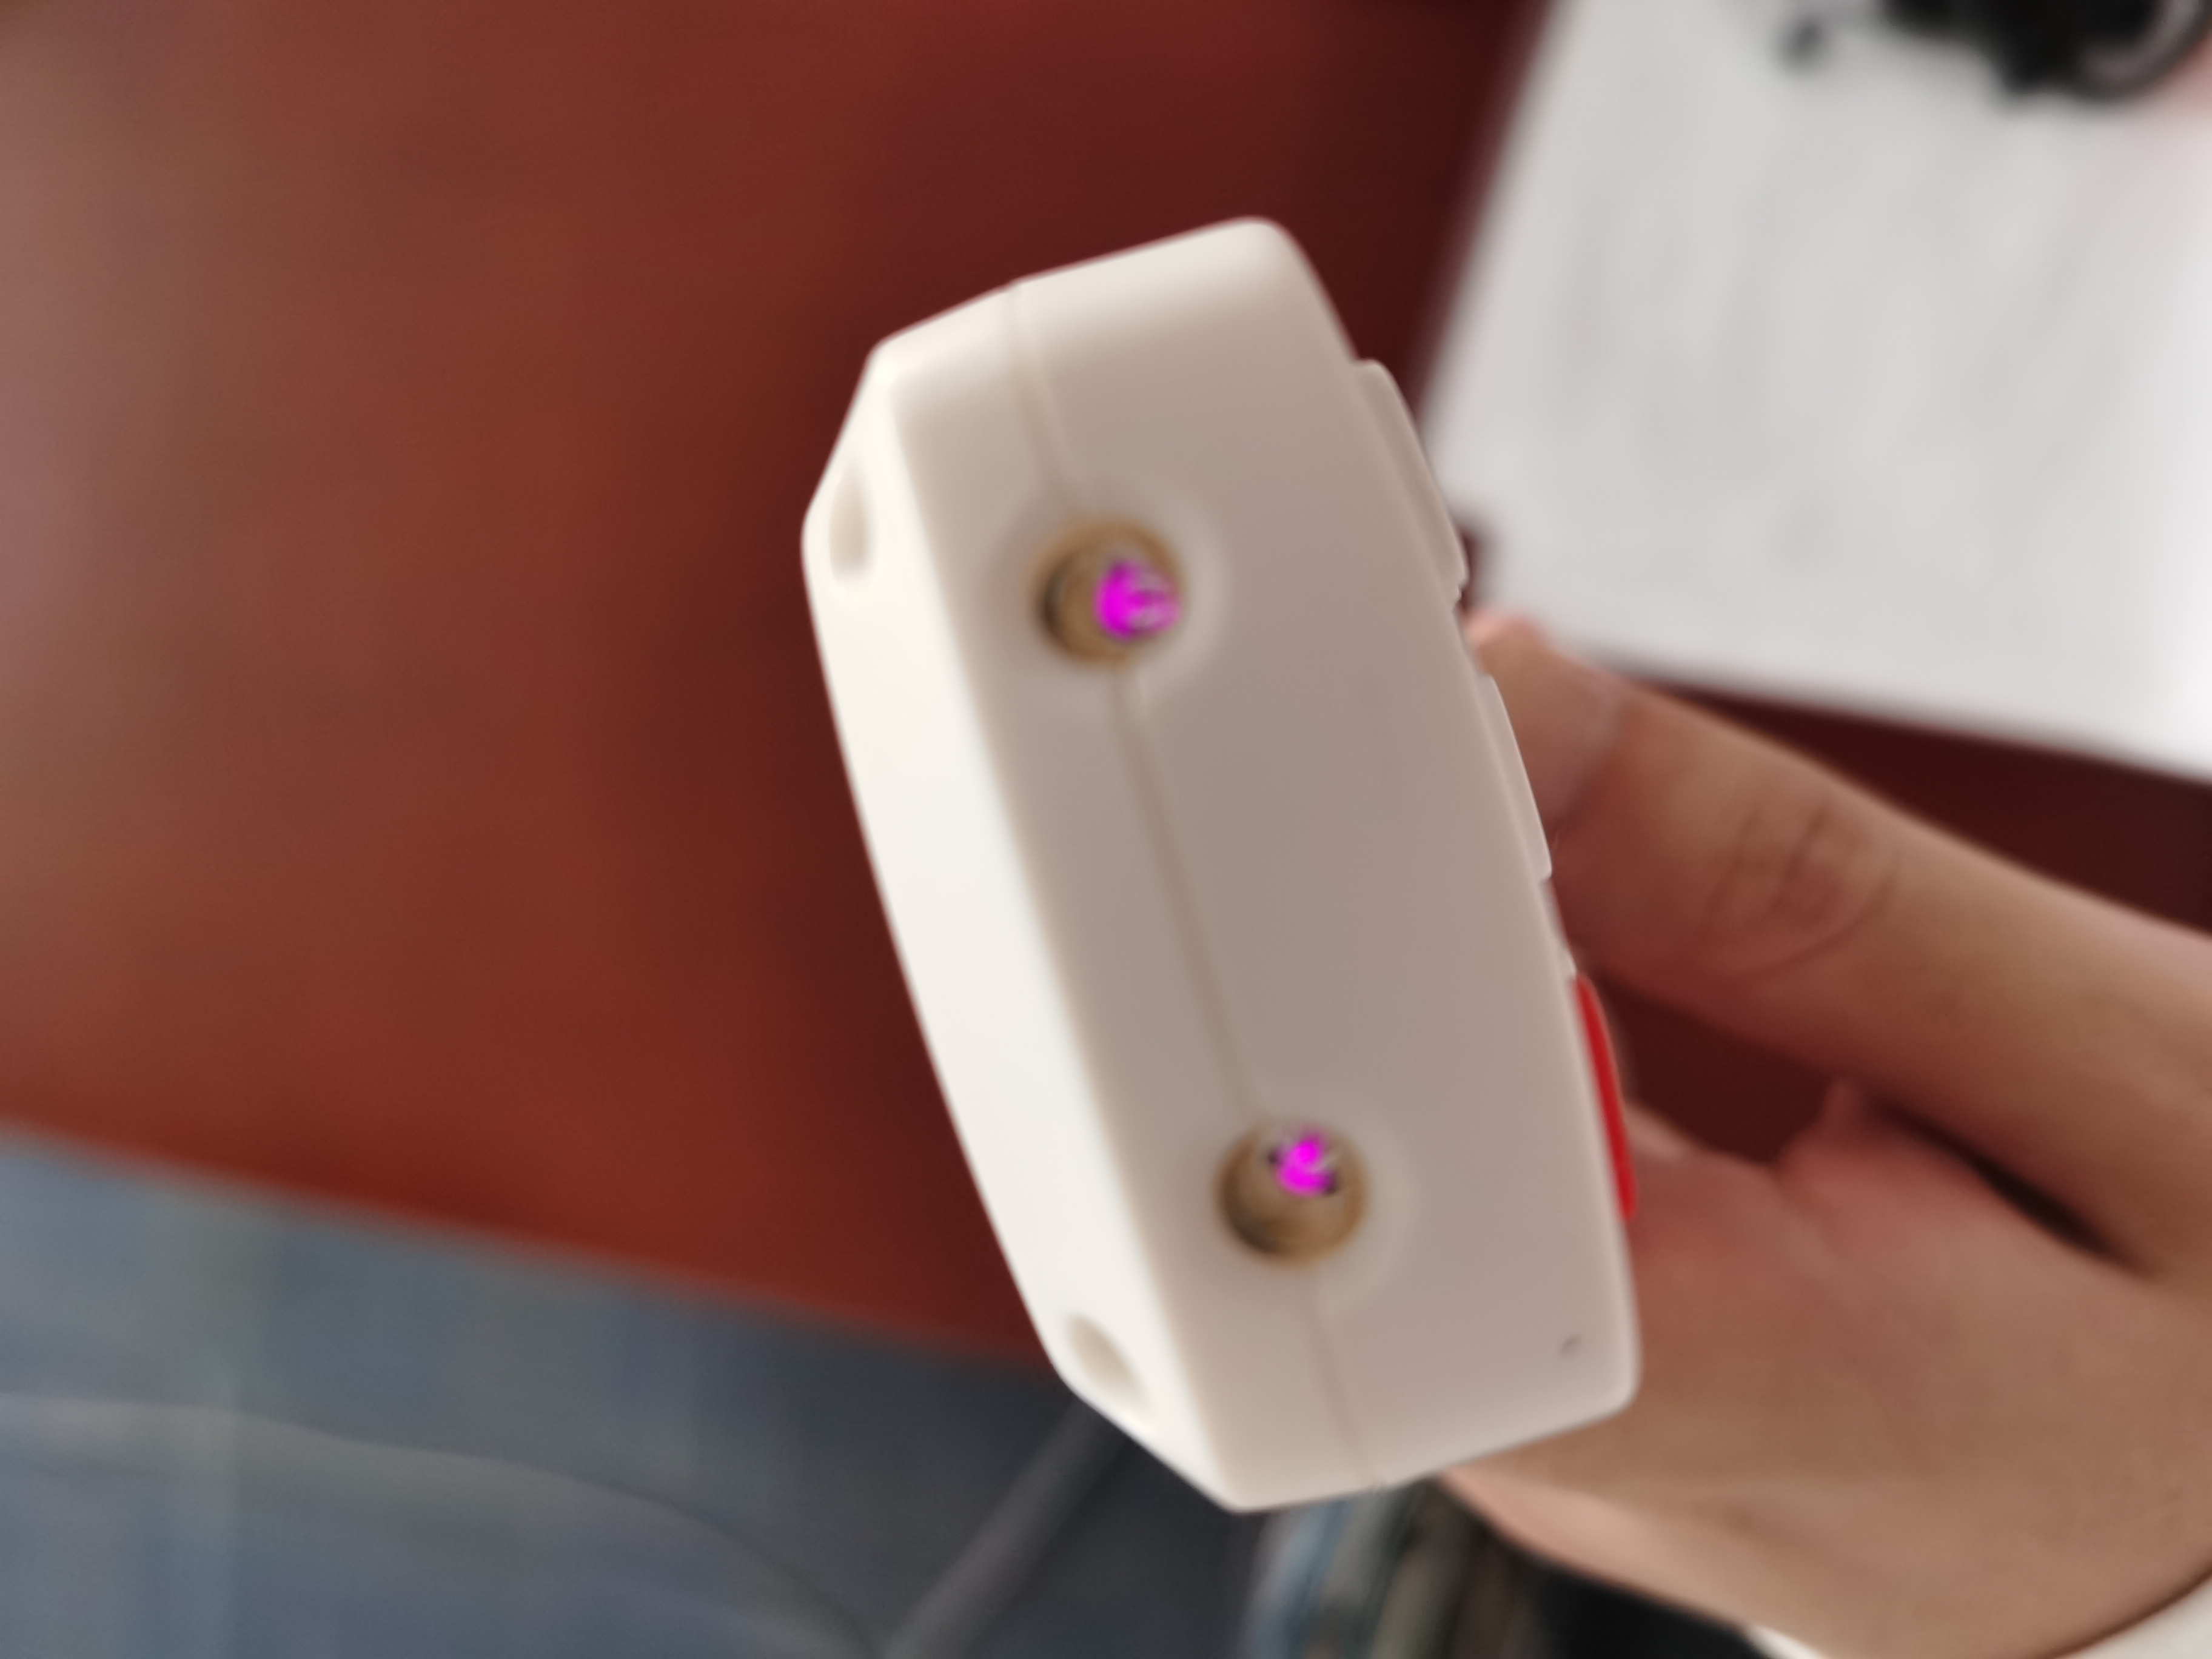
\includegraphics[width = 120mm]{infrared-ray-lamp.jpeg}
	\caption{手机拍摄红外遥控器照片}
\end{figure}

\end{enumerate}

\end{document}